\chapter{Retrieval and Optimization Methods}
\label{chap:retrieval_optimization}

The retrieval component is the heart of a RAG system. Its ability to surface high-quality, relevant information from a vast corpus is the primary determinant of the system's overall performance. This chapter provides a detailed exploration of the critical techniques used to build and optimize the retrieval pipeline, from the initial processing of documents to the final reranking of retrieved candidates. We will follow the structure proposed by Gao et al. (2024) \autocite{gao2024retrievalaugmented}, which categorizes RAG optimization into pre-retrieval, retrieval, and post-retrieval stages.

\section{Chunking Techniques}
Chunking is a key pre-retrieval processing step that involves breaking down large documents into smaller, more manageable pieces. The goal is to create chunks that are semantically coherent and small enough to be efficiently processed by embedding models and fit within the context window of an LLM. The choice of chunking strategy has a profound impact on retrieval quality.

\subsection{Naive vs. Semantic Chunking}
\textbf{Naive Chunking}, also known as fixed-size chunking, is the simplest approach. It involves splitting documents into segments of a predetermined length (e.g., 200 words) with an optional overlap between adjacent chunks. While easy to implement, this method can be suboptimal as it often splits sentences or paragraphs in the middle, breaking the semantic continuity of the text.

\textbf{Semantic Chunking} represents a more sophisticated approach. Instead of relying on arbitrary lengths, it aims to divide the text at logical boundaries. This can be done in several ways:
\begin{itemize}
    \item \textbf{Sentence-Level Chunking:} Using natural language processing libraries to split the text into individual sentences.
    \item \textbf{Recursive Chunking:} A hierarchical method that first tries to split by paragraphs, then by sentences, and finally by words, to maintain semantic coherence as much as possible.
    \item \textbf{Agentic Chunking:} Employing an LLM to analyze the document and decide the most appropriate chunking strategy based on the content's structure and nature.
\end{itemize}

\section{Embedding Models}
The choice of embedding model is critical for capturing the semantic meaning of the text. These models transform text into high-dimensional vectors, where semantically similar texts are located closer to each other in the vector space.

\subsection{Contextual Embeddings}
Modern RAG systems rely on \textbf{contextual embeddings}, such as those produced by transformer-based models like BERT, RoBERTa, and the OpenAI Ada series. Unlike older static word embeddings (e.g., Word2Vec, GloVe), which assign a single vector to each word, contextual embeddings generate a unique vector for a word based on the sentence it appears in. This allows them to capture nuances, ambiguity, and the richness of language, leading to more accurate semantic search.

\subsection{Fine-tuning Embedding Models}
For domain-specific applications, pre-trained embedding models may not perform optimally. Fine-tuning the embedding model on a dataset that is representative of the target domain can significantly improve retrieval relevance. This process adapts the model to the specific vocabulary and semantic relationships present in the corpus.

\section{Post-Retrieval Reranking and Filtering}
Once an initial set of documents is retrieved based on semantic similarity, their relevance and ordering can be further improved through post-retrieval processing. This is a key component of the \textbf{Advanced RAG} paradigm \autocite{gao2024retrievalaugmented}.

\subsection{BM25 and TF-IDF for Reranking}
Traditional information retrieval algorithms like \textbf{BM25} and \textbf{TF-IDF} are based on keyword matching. They are highly effective at finding documents that contain the exact keywords from the query. While dense retrievers (vector search) find what the user \textit{means}, these sparse retrievers find what the user \textit{says}. By using BM25 or TF-IDF to rerank the candidates retrieved by vector search, we can improve precision by boosting the rank of documents that have high lexical overlap with the query \autocite{gao2024retrievalaugmented}.

\subsection{Hybrid Systems: Combining Similarity with BM25/TF-IDF}
A fully \textbf{hybrid system} combines the scores from both dense (semantic) and sparse (keyword) retrieval methods from the outset. A common approach is to use a weighted combination of the scores from a vector search and a BM25 search to produce a final relevance score. This allows the system to leverage the strengths of both approaches, capturing both semantic relevance and keyword importance for a more robust retrieval process \autocite{gao2024retrievalaugmented}.

\subsection{Cross-Encoder Rerankers}
For the highest possible accuracy, a \textbf{cross-encoder} model can be used as a final reranking step. Unlike bi-encoders (standard embedding models) that create separate embeddings for the query and documents, a cross-encoder takes the query and a candidate document as a single input. This allows the model to perform a deep, token-by-token comparison, resulting in a highly accurate relevance score \autocite{khattab2020colbert}. However, cross-encoders are computationally expensive and are typically only used to rerank a small number of top candidates from a faster, initial retrieval stage.

\section{Dynamic Similarity Thresholding}
Instead of retrieving a fixed number of chunks (top-N), \textbf{dynamic similarity thresholding} adapts the retrieval process based on the query itself. For some queries, only a few highly relevant chunks may be needed, while for others, a broader context is beneficial. Dynamic thresholding methods analyze the distribution of similarity scores for a given query and attempt to find a natural cutoff point, helping to retrieve a more contextually appropriate number of chunks. This prevents the inclusion of irrelevant documents when the similarity scores drop off sharply and allows for more comprehensive retrieval when many documents are similarly relevant.

\section{Late Chunking with Contextual Chunk Embeddings}
Late chunking is an advanced strategy that fundamentally changes how chunk embeddings are generated, moving away from the isolated processing of chunks to a more holistic, context-aware approach. As detailed by Günther et al. (2025) \autocite{günther2025latechunkingcontextualchunk}, this technique leverages the full power of long-context embedding models to create what they term \textit{Contextual Chunk Embeddings}.

\subsection{Limitations of Traditional Chunking}
In a traditional chunking workflow, a document is first split into discrete chunks (e.g., by paragraphs or fixed token counts or for each page or by a different chunking strategy). Then, an embedding model is applied to each chunk independently to generate its vector representation. The major drawback of this method is context loss. The embedding for each chunk is created in a vacuum, unaware of the preceding or succeeding information in the original document. This can lead to ambiguous or less meaningful embeddings, thereby degrading the quality of the retrieval process, as the model cannot capture the full semantic richness of the text.

\subsection{The Late Chunking Process}
Late chunking addresses this limitation by reversing the process: it first generates highly contextualized embeddings at the token level and only then applies chunk boundaries. The process, detailed in Algorithm \ref{alg:late_chunking}, is as follows:

\begin{enumerate}
    \item \textbf{Tokenization and Contextualization:} Instead of chunking the document first, the entire document (or the largest possible segment that fits into the model's context window) is tokenized. The transformer model then processes this long sequence of tokens, generating a vector representation ($\omega_i$) for every single token. Crucially, each of these token embeddings is context-aware, as it was created with knowledge of the entire surrounding text.

    \item \textbf{Boundary Cue Application:} After the token-level embeddings ($\omega_1, \dots, \omega_m$) have been generated, the predefined chunk boundaries are used. These boundaries, which are determined by a standard chunking algorithm (e.g., sentence splitting), are not used to split the text for the model, but rather to identify which token embeddings correspond to which chunk. This is the key step from which the technique derives its name: the chunking logic is applied \textit{late} in the process.

    \item \textbf{Pooling:} With the token embeddings for each chunk identified, a pooling function—typically mean pooling—is applied to the sequence of token vectors within each chunk's boundaries. This aggregates the contextualized token embeddings into a single, final vector for each chunk.
\end{enumerate}

This "inside-out" approach ensures that the final embedding for each chunk is not just a representation of the text within it, but is deeply informed by the broader context of the entire document, leading to more robust and accurate retrieval.

The concept of late chunking was introduced by Jina AI with the release of their \texttt{jina-embeddings-v2} model family. It has since been refined and extended in subsequent releases, including \texttt{jina-embeddings-v3} \autocite{sturua2024jinaembeddingsv3multilingualembeddingstask} and \texttt{jina-embeddings-v4} \autocite{günther2025jinaembeddingsv4universalembeddingsmultimodal}. While the later versions introduced multimodal capabilities, which are not the focus of this study, the core principle of late chunking for text remains a key innovation.

\begin{figure}[!htbp]
    \centering
    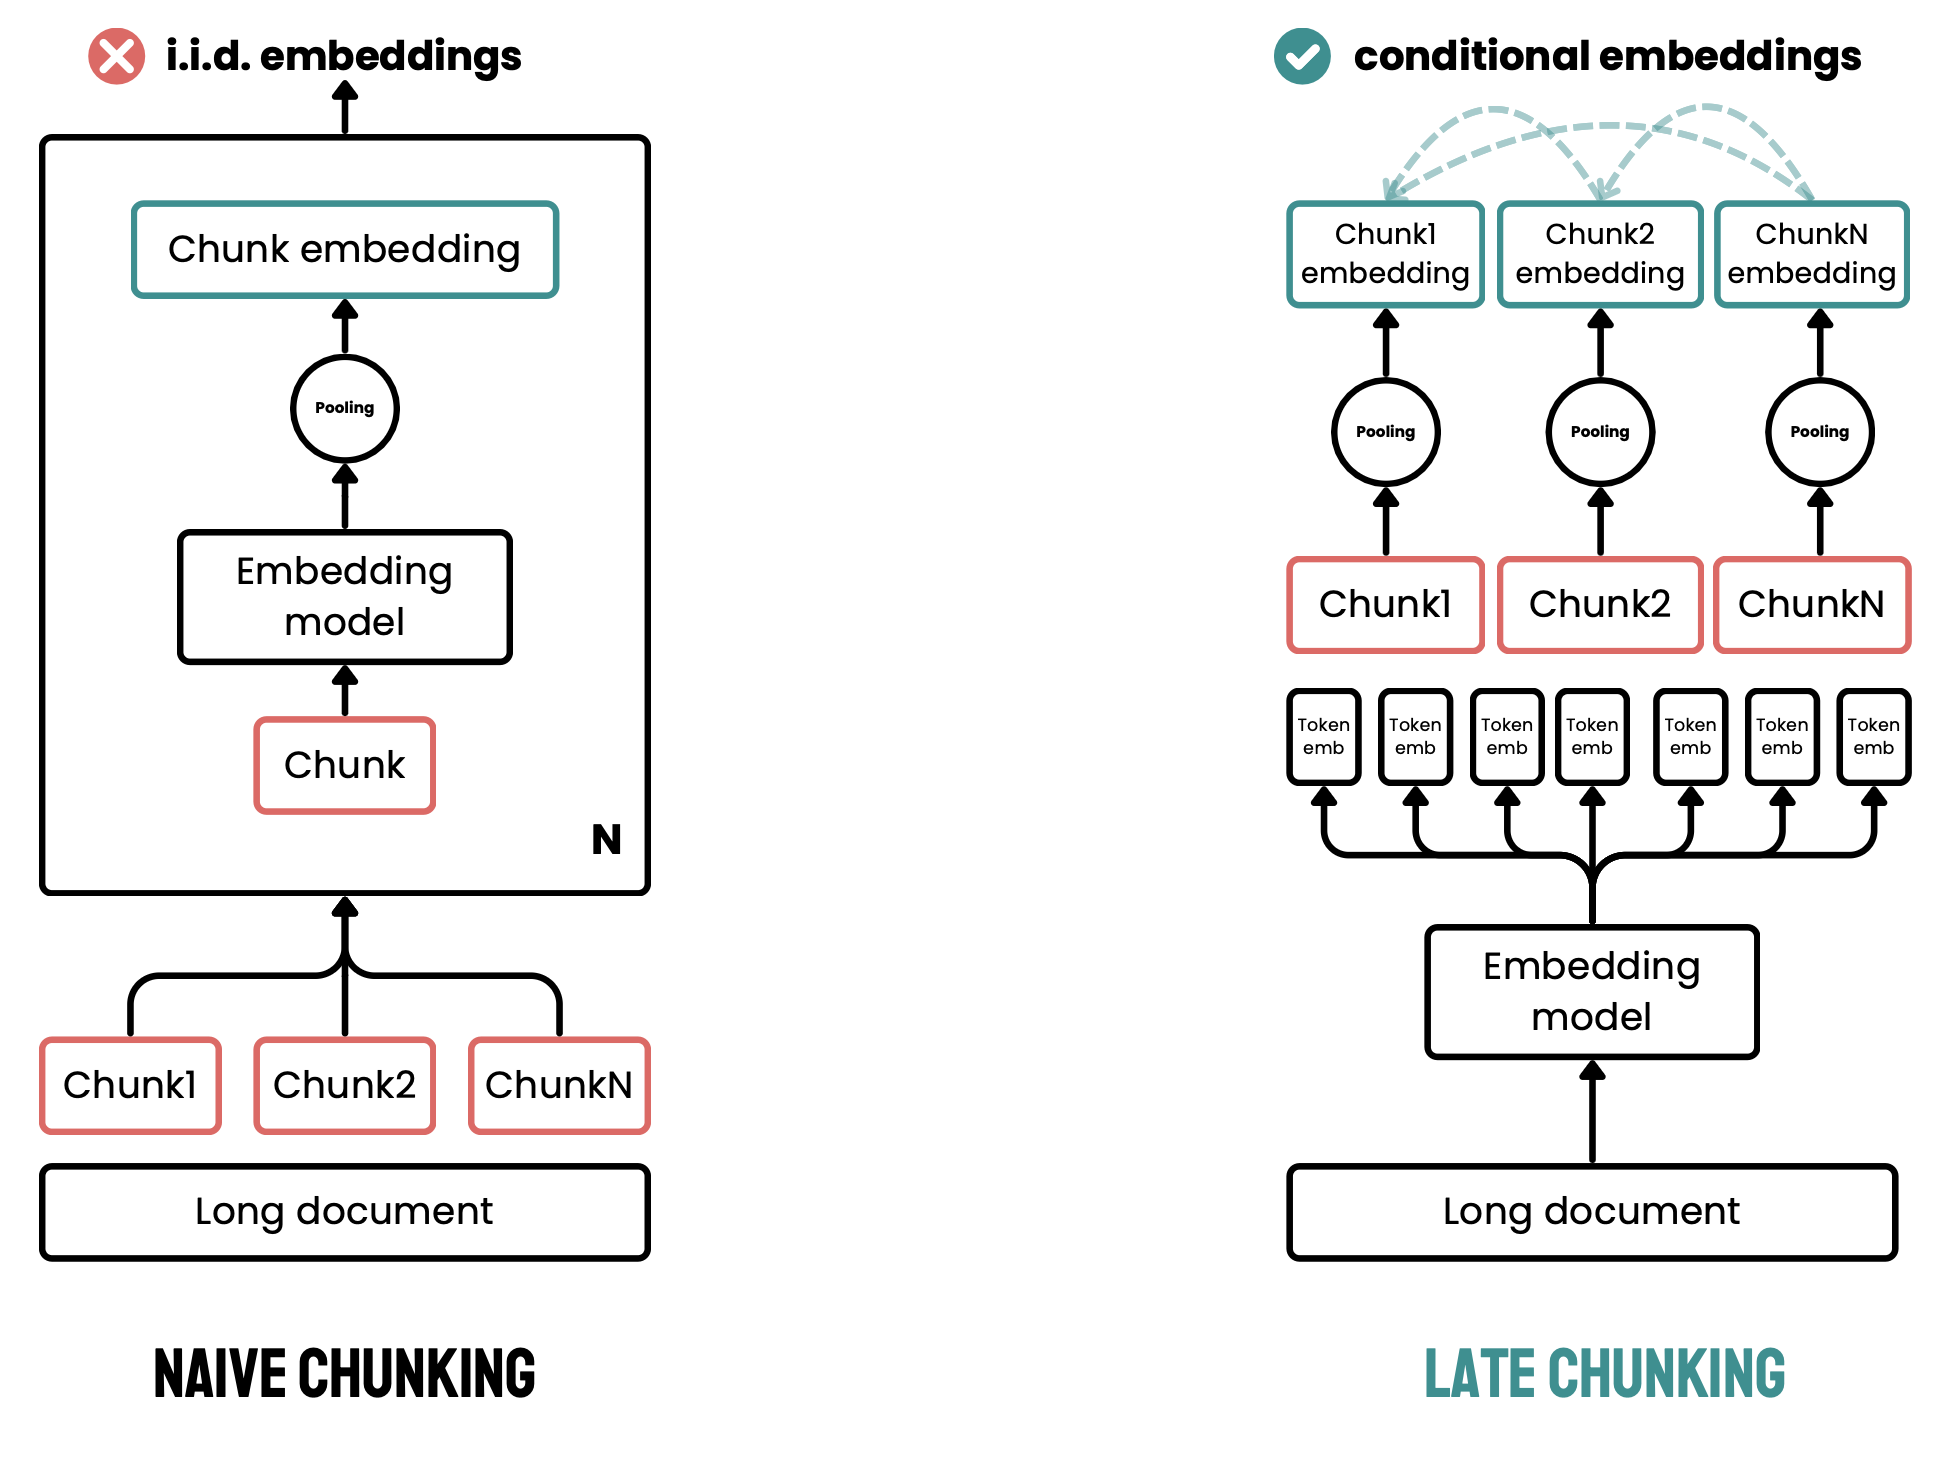
\includegraphics[width=\textwidth]{images/chapter3/late_chunking.png}
    \caption{Visualization of the Late Chunking algorithm (right) compared to naive chunking (left). Image from Günther et al. (2025) \autocite{günther2025latechunkingcontextualchunk}.}
    \label{fig:late_chunking}
\end{figure}

\begin{algorithm}
\caption{Late Chunking}
\label{alg:late_chunking}
\begin{algorithmic}[1]
\Procedure{LateChunking}{document, chunk\_boundaries}
    \State $tokens \gets \text{tokenize}(document)$
    \State $\omega_1, \dots, \omega_m \gets \text{Transformer}(tokens)$ \Comment{Generate token-level embeddings}
    \State $token\_spans \gets \text{get\_token\_spans}(document, tokens)$
    \State $chunk\_token\_indices \gets []$
    \For{each $chunk$ in $chunk\_boundaries$}
        \State $start\_char, end\_char \gets chunk$
        \State $start\_token \gets \text{find\_token\_at\_char}(token\_spans, start\_char)$
        \State $end\_token \gets \text{find\_token\_at\_char}(token\_spans, end\_char)$
        \State append $(start\_token, end\_token)$ to $chunk\_token\_indices$
    \EndFor
    \State $chunk\_embeddings \gets []$
    \For{each $start\_idx, end\_idx$ in $chunk\_token\_indices$}
        \State $token\_vectors\_for\_chunk \gets \omega_{start\_idx}, \dots, \omega_{end\_idx}$
        \State $embedding \gets \text{MeanPool}(token\_vectors\_for\_chunk)$
        \State append $embedding$ to $chunk\_embeddings$
    \EndFor
    \State \Return $chunk\_embeddings$
\EndProcedure
\end{algorithmic}
\end{algorithm}